	%  this is a description of a cvd process usually used in this work
There are many ways to grow ad layers with controlled stoichiometry in UHV. Here we will only focus on the most used method for sub mono layer and mono layer growth - the chemical vapor deposition (CVD). 
%#####################################################
\begin{figure}\centering
	\subfigure[Diboran and ammonia]{
		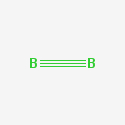
\includegraphics[width=0.05\textwidth]{./images/precursor/diboran-125x125}
		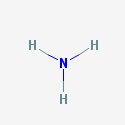
\includegraphics[width=0.05\textwidth]{./images/precursor/ammonia-125x125}
		\label{fig:diboran-ammonia}
	} \qquad%
	\subfigure[Ammonia borane]{
		\includegraphics[width=0.05\textwidth]{./images/precursor/ammonia-borane-125x125}
		\label{fig:ammonia-borane}
	} \qquad%
	\subfigure[Borazine]{
		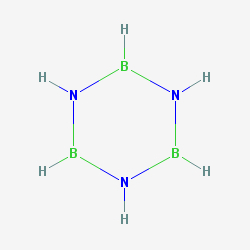
\includegraphics[width=0.1\textwidth]{./images/precursor/borazine-250x250}
		\label{fig:borazine}
	} \qquad%
	\subfigure[Trichloroborazine]{
		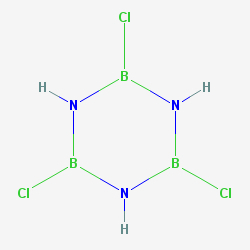
\includegraphics[width=0.1\textwidth]{./images/precursor/B-Trichloroborazine-250x250}
		\label{fig:B-Trichloroborazine}
	} \qquad%
	\subfigure[Decaborane ammonia]{
		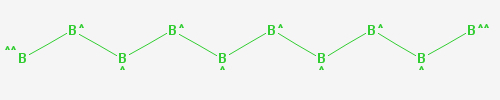
\includegraphics[width=0.2\textwidth]{./images/precursor/decaborane-500x100}
		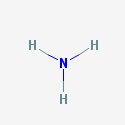
\includegraphics[width=0.05\textwidth]{./images/precursor/ammonia-125x125}
		\label{fig:decaborane-ammonia}
	} \qquad%
	\caption{Precursor molecules for \textit{h}-BN growth. \subref{fig:diboran-ammonia} A mixture of ammonia and diborane, \subref{fig:ammonia-borane} ammonia borane, \subref{fig:borazine} borazine and \subref{fig:B-Trichloroborazine} B-Trichloroborazine, \subref{fig:decaborane-ammonia} a mixture of decaborane and ammonia. Images reproduced from \cite{_pubchem}}
	\label{fig:h-BN-precursor}
\end{figure}
%#####################################################

When a gaseous precursor comes on contact with a hot transition metal surface, the precursor is split by pyrolysis into fragments. These then distribute across the surface and form new structures in a self-organized process. Choosing the right growth parameters like temperature, precursor partial pressure and time, high quality layers can be grown, whose stoichiometry is determined by the chemical structure of the precursor. Using carbon rich gases like ethylene (C2H4) \cite{ndiaye_structure_2008-1, coraux_growth_2009} and coronene (C24H12) \cite{coraux_growth_2009} as precursor and a transition metal as substrate results in a graphene layer to be formed. Using boron and nitrogen containing molecules (see \autoref{fig:h-BN-precursor})
\footnote{\textit{h}-BN CVD precursor:
	
	Borazine \cite{muller_epitaxial_2010, joshi_boron_2012, schwarz_corrugation_2017, li_grain_2015, preobrajenski_monolayer_2005, auwarter_xpd_1999, morscher_formation_2006, preobrajenski_monolayer_2007-1, corso_boron_2004, goriachko_self-assembly_2007, kidambi_situ_2014, kim_synthesis_2012}
	
	B-Trichloroborazine (${ClBNH}_3$) \cite{auwarter_synthesis_2004-1, muller_symmetry_2005}
	
	Ammonia borane (borazane) \cite{guo_controllable_2012-4, lee_large-scale_2012, kim_synthesis_2012-1} 
	
	Diborane and ammonia \cite{ismach_toward_2012}
	
	Reaction of ammonia with decaborane \cite{chatterjee_chemical_2011}
	
	Triethylborane and ammonia \cite{siegel_heterogeneous_2017}
} 
as precursor will result in \textit{h}-BN to be formed. Hereby either single crystalline \footnote{Single crystals used as growth substrate for \textit{h}-BN:
	
	(111):
	Ag \cite{muller_epitaxial_2010}, 
	Cu \cite{joshi_boron_2012, schwarz_corrugation_2017, li_grain_2015, preobrajenski_monolayer_2005,siegel_heterogeneous_2017}, 
	Ni \cite{preobrajenski_monolayer_2005, nagashima_electronic_1995, auwarter_synthesis_2004-1, auwarter_xpd_1999}, 
	Rh \cite{preobrajenski_monolayer_2007-1, corso_boron_2004},
	Pd \cite{nagashima_electronic_1995, morscher_formation_2006}, 
	Pt \cite{nagashima_electronic_1995, preobrajenski_monolayer_2007-1, muller_symmetry_2005}, 
	
	others:
	Cu(100) \cite{guo_controllable_2012-4}, 
	Ru(0001) \cite{goriachko_self-assembly_2007, preobrajenski_monolayer_2007-1}
}
or polycrystalline foils \footnote{Polycrystalline foils used as substrate:
	
	Cu: \cite{kidambi_situ_2014, lee_large-scale_2012, kim_synthesis_2012, kim_synthesis_2012-1, ismach_toward_2012, guo_controllable_2012-4, chatterjee_chemical_2011}
	
	Ni: \cite{ismach_toward_2012, chatterjee_chemical_2011}
}
are used as substrates. These play a key role in interaction strength with the ad layer. Their lattice constant determines the mismatch with the ad layer. For some of these systems, DFT calculation back up experimental results \cite{gomez_diaz_hexagonal_2013}.

\paragraph{self-limitation}
The precursors decomposes on contact with the hot substrate surface and its fragments form the ad layer. As time goes by, the ad layer grows in coverage and less free hot surface area is available for decomposing new ``building blocks'' for mono layer formation. If a mono layer is formed, no additional second layer is formed because of missing building blocks which only arise on contact with the uncovered substrate surface. Therefore this process is called self-limited. It is observed \cite{corso_h-bn_2005, cavar_single_2008, muller_epitaxial_2010} for various substrates in combination with a borazine precursor.

%While in CVD, the process of forming the ad layer (adsorption, decomposing, diffusion on surface upon coalescence with an already present nucleation seed, layer growth), \textbf{TPG} offers some other path of layer growth. 
%
%Due to the fact that the surface is covered from the beginning with the desired number of molecules, the density of present building blocks at a certain time (and same dosage as with CVD) is higher. Therefore this growth experiences other results as CVD. In direct comparison CVD has been a better way to grow full mono layers \cite{coraux_growth_2009}.

%	Hexagonal boron nitride grown on transition metals shows distinct differences between these two modes. CVD results in a more homogeneous mono layer coverage than TPG and is therefore preferred.
%

The growth by itself is well investigated on transition metal surfaces \cite{gomez_diaz_hexagonal_2013,morscher_formation_2006}, on the copper and nickel surfaces \cite{preobrajenski_monolayer_2005,joshi_boron_2012}. Even more complicated samples can be created with this technique \cite{roth_chemical_2013} and the following gives a short introduction in the occurring growth processes.

Some growth mechanics can be seen best in figure \ref{fig:borazine-TPG-on-Ir} that shows a XPS spectrum of borazine adsorbed on a Iridium surface held at \SI{170}{\kelvin} and after several annealing steps. 

At the graphics' bottom one can see the clean Ir surface with no borazine adsorbed (no B1s signal ). There are two contributions in the Ir-peak. While the low energy ($Ir_s$) peak stems from the surface atoms of the substrate, $Ir_b$ denotes the contribution from the atoms in the bulk. Upon borazine adsorption $(1)$ a broad $B1s$ emerges accompanied with a new contribution in the $Ir$-peak ($Ir_i$) which is a result of borazine-Ir interaction decreasing the area of $I_b$ and $I_s$ .
Upon annealing ($(2)$-$(6)$) $Ir_i$ looses in intensity while the $I_b$ and $I_s$ recover to their initial position. Interesting changes happen to the $B1s$ peak. While at lower temperatures, several peak contributions can be distinguished, denoted as $B_{mol}$ for entire molecules and $B_{ad}$ for molecular fragments. With increasing temperature, $B_{mol}$ decreases for a increase in the $B_0$ peaks. At lower temperature (1), $B_{mol}$ decreases and $B_{ad}$ slightly increases. 
\begin{wrapfigure}{l}{0.3\textwidth}\centering
	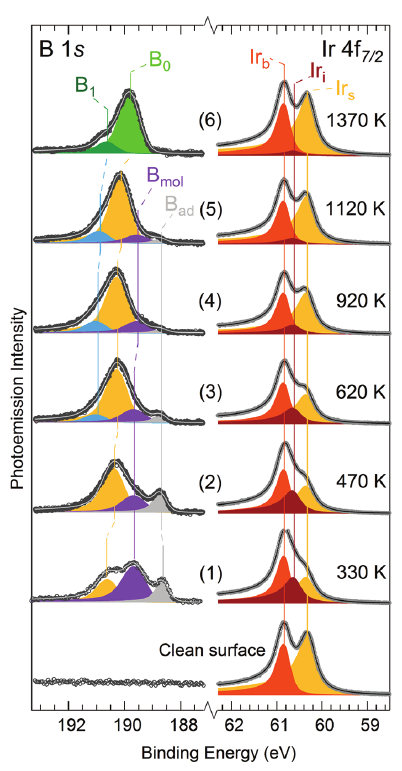
\includegraphics[width=0.3\textwidth]{./images/07571n_fig5.png}
	\caption{RT XPS spectra (B1s and Ir4f 7/2) of borazine adsorbed on a Iridium surface held at \SI{170}{\kelvin} and after stepwise annealing to \SI{1370}{\kelvin}. Adopted from \cite{orlando_epitaxial_2012}}
	\label{fig:borazine-TPG-on-Ir}
\end{wrapfigure}
When exceeding 620K ($\approx \SI{350}{\celsius}$, (3)) a new peak emerges and develops into $B_1$ when increasing temperatures. When temperature is high enough the only peaks left are $B_0$ and $B_1$ - the two contributions of boron atoms stem from boron atoms interact with the Iridium substrate with different strength due to different registry to the substrate.

While the growth temperature and partial pressures used to grow defect free \textit{h}-BN layers varies, the basic principle remains the same on all substrates.

The exact growth of mono- and multi layers \cite{ismach_toward_2012} is prone to discussion and may involve  
